\chapter{ADM}


\section{Introdución}

TOGAF ADM (Architecture Development Method) forma el centro de TOGAF. ADM es el resultado de contribuciones continuas de un gran número de arquitecturas, también describe un método para desarrollar y administrar el ciclo de vida de una arquitectura empresarial, ademas se apoya en muchos de los elementos de TOGAF y recursos de otras arquitecturas que están disponibles con el fin de conocer el negocio y las TI que de una organización.
\newline
El framework de TOGAF se complementa de Archimate puesto que este proporciona un conjunto independiente de conceptos, incluyendo una representación gráfica, que ayuda a crear un modelo coherente e integrado  "por debajo de la linea de flotación" que se puede representar en forma de vistas TOGAF, es por eso que en el desarrollo de este capitulo se explicara el uso de ADM, sus puntos claves y las integración que se da con Archimate desde las diferentes capas que este tiene.

\newpage

\section{Arquitectura base de una empresa}

ADM es útil para describir la Arquitectura Base de una empresa. Los requisitos empresariales que se tienen se pueden utilizar para identificar las definiciones y selecciones necesarias en la base de la arquitectura. Estos requisitos pueden ser un conjunto de modelos comunes reutilizables, políticas y definiciones de gobernabilidad, o incluso pueden ser algo mas especifico como selecciones tecnológicas sobresaliente. Al realizar la descripción de la Arquitectura Base se sigue principios similares a los de una arquitectura empresarial, con la diferencia de que los requisitos para toda una empresa se limitan a las preocupaciones generales y, por tanto, es menos completo que para una parte de la empresa específica.

\subsection{Puntos clavede ADM}

\begin{itemize}
	\item ADM es iterativo, a lo largo de todo el proceso, entre las fases, y dentro de las fases . Para cada interacción de la ADM, una nueva decisión debe ser tomada en base a:
	\begin{itemize}
		\item La amplitud de la cobertura de la empresa que se define.
		\item El nivel de detalle que se define.
		\item La extensión del período de tiempo destinado, incluyendo el número y la extensión de los períodos de tiempo intermedios.
		\item Los activos de arquitectura para ser aprovechados, incluyendo:
		\begin{itemize}
			\item Activos creados en versiones anteriores del ciclo de ADM dentro de la empresa.
			\item Activos disponibles en otras partes de la industria (otros marcos, modelos de sistemas, modelos verticales de la industria, etc.).
		\end{itemize}
	\end{itemize}
	\item Las decisiones tomadas en cada fase se deben basar en una evaluación práctica de los recursos y la disponibilidad de competencias, y en el valor que realmente se puede esperar recibir de la empresa en el ámbito elegido del trabajo de la arquitectura.
	\item Como un método genérico, ADM está destinado a ser utilizado por empresas en una amplia variedad de diferentes zonas geográficas y aplicado en diferentes tipos sectores / industria vertical. Como tal, puede ser, pero no necesariamente tiene que ser, adaptado a las necesidades específicas.
\end{itemize}

\newpage
\subsection{Modelo de proceso ADM}

Es importante recalcar que a lo largo del ciclo ADM, es necesario que se evaluen los resultados contra las expectativas originales, esto tanto para el ciclo ADM completo como para cada fase particular del proceso. \cite{togaf2}

\begin{figure}[h]
	\centering
	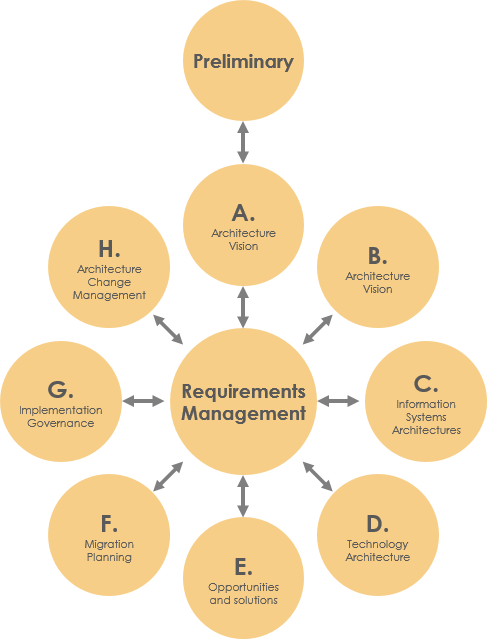
\includegraphics[width=0.7\linewidth]{arquitectura/imagenes/modeloADM}
	\caption{Estructura base del Modelo de Proceso de ADM }
	\label{fig:modeloadm}
\end{figure}
\newpage


\section{ArchiMate}

ArchiMate es un lenguaje de modelado de arquitectura empresarial abierto e independiente que soporta la descripción, análisis y visualización de las relaciones entre los diferentes dominios de negocios de una forma no ambigua, es deccir, la especificación de ArchiMate define un lenguaje común para describir la construcción y operación de procesos de negocios, estructuras organizacionales, flujos de información, sistemas de TI e infraestructura técnica. Esta visión ayuda a las partes interesadas a diseñar, evaluar y comunicar las consecuencias de las decisiones y cambios dentro y entre los dominios de negocio.  
\newline
Con su versión mas reciente ArchiMate 3.0 de 2016, se puede modelar la empresa a un nivel estratégico, como capacidad, recursos y resultados. También se incluye el apoyo para modelar el mundo físico de materiales y equipos.
\newline
ArchiMate se divide en capas como se puede observar en la siguiente figura:
\newline

\begin{figure} [h]
	\centering
	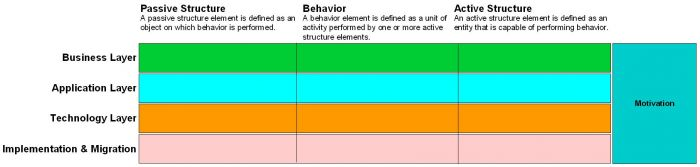
\includegraphics[width=0.7\linewidth]{arquitectura/imagenes/Archimate}
	\caption{Estructura por capas de ArchiMate \cite{togaf1}}
	\label{fig:archimate}
\end{figure}

A continuación se van a mostrar los conceptos de las diferentes capas que se utilizan para el modelamiento en ArchiMate \cite{togaf4}, dentro de las que se encuentran Capa de Negocio, Capa de Aplicación, Capa de Tecnologías, Capa de Motivación y Capa de Migración, además de esto también se mostrara la tabla de Relaciones.

\newpage

\subsection{Capa de negocio}

Se refiere a los procesos de negocio, servicios, funciones y eventos ce cada una de las unidades de negocio. Esta capa ofrece productos y servicios a clientes externos, que se realizan en la organización mediante procesos de negocio realizados por actores y roles empresariales.

\begin{table}[H]
	\centering\textbf{TABLA DE CONCEPTOS CAPA DE NEGOCIO}

	\centering
	\begin{tabular}{| m{4cm} | m{4cm} | m{4cm} | }
		\hline
		\centering\vspace{1.52mm}CONCEPTO & \centering\vspace{1.52mm}DESCRIPCION & \vspace{1.52mm}NOTACION \\
		\hline
		\centering\vspace{1.52mm}Actor de Negocio & \vspace{1.52mm} Una entidad de organización que es capaz de comportamiento artístico. & \vspace{1.52mm}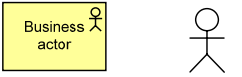
\includegraphics[width=40mm]{arquitectura/imagenes/11} \\
		\hline
		\centering\vspace{1.52mm}Rol de Negocio & \vspace{1.52mm} La responsabilidad de realizar el comportamiento específico, al cual un actor puede ser asignado.  & \vspace{1.52mm}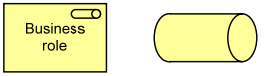
\includegraphics[width=40mm]{arquitectura/imagenes/12} \\
		\hline
		\centering\vspace{1.52mm}Colaboración de Negocio & \vspace{1.52mm}Un conjunto de dos o más papeles de negocio que trabajan juntos para realizar el comportamiento colectivo.   & \vspace{1.52mm}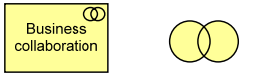
\includegraphics[width=40mm]{arquitectura/imagenes/13} \\
		\hline
		\centering\vspace{1.52mm}Interfaz de Negocio & \vspace{1.52mm}Un punto de acceso donde un servicio de gestión es hecho disponible al entorno.   & \vspace{1.52mm}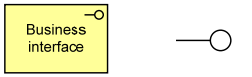
\includegraphics[width=40mm]{arquitectura/imagenes/14} \\
		\hline
		\centering\vspace{1.52mm}Ubicación & \vspace{1.52mm}Un punto conceptual o ampliado en espacio.& \vspace{1.52mm}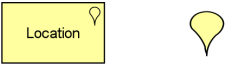
\includegraphics[width=40mm]{arquitectura/imagenes/15} \\
		\hline
		\centering\vspace{1.52mm}Objeto de Negocio & \vspace{1.52mm}Un elemento pasivo que tiene la importancia de una perspectiva de negocio. & \vspace{1.52mm}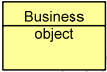
\includegraphics[width=20mm]{arquitectura/imagenes/16} \\
		\hline
		\centering\vspace{1.52mm}Proceso de Negocio & \vspace{1.52mm}Un elemento de comportamiento de grupos basado en un ordenamiento de actividades. Es querido para producir un juego definido de productos o servicios de gestión. & \vspace{1.52mm}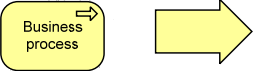
\includegraphics[width=40mm]{arquitectura/imagenes/17} \\
		\hline
		\centering\vspace{1.52mm}Función de Negocio & \vspace{1.52mm}Un elemento de comportamiento de grupos basado en un juego escogido de criterios (recursos típicamente requeridos de negocio y/o competencias).  & \vspace{1.52mm}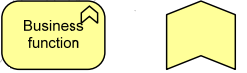
\includegraphics[width=40mm]{arquitectura/imagenes/18} \\
		\hline
	\end{tabular}
\end{table}

\begin{table}[H]
	\centering
	\begin{tabular}{| m{4cm} | m{4cm} | m{4cm} | }
		\hline
		\centering\vspace{1.52mm}CONCEPTO & \centering\vspace{1.52mm}DESCRIPCION &\vspace{1.52mm}NOTACION \\
		\hline
		\centering\vspace{1.52mm}Interacción de Negocio & \vspace{1.52mm}Un elemento de comportamiento que describe el comportamiento de una colaboración de negocio.   & \vspace{1.52mm}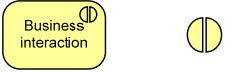
\includegraphics[width=40mm]{arquitectura/imagenes/19} \\
		\hline
		\centering\vspace{1.52mm}Evento de Negocio & \vspace{1.52mm}Algo qué pasa (internamente o por fuera) e influye en el comportamiento. & \vspace{1.52mm}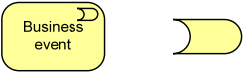
\includegraphics[width=40mm]{arquitectura/imagenes/110} \\
		\hline
		\centering\vspace{1.52mm}Servicio de Negocio & \vspace{1.52mm}Un servicio que realiza una necesidad de negocio de un cliente (interno o externo a la organización). & \vspace{1.52mm}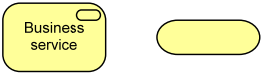
\includegraphics[width=40mm]{arquitectura/imagenes/111} \\
		\hline
		\centering\vspace{1.52mm}Representación & \vspace{1.52mm}Una forma perceptible de la información llevada por un objeto de negocio. & \vspace{1.52mm}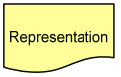
\includegraphics[width=20mm]{arquitectura/imagenes/112} \\
		\hline
		\centering\vspace{1.52mm}Significado & \vspace{1.52mm}El conocimiento o la experiencia se presentan en un objeto de negocio o su representación, considerando un contexto particular. & \vspace{1.52mm}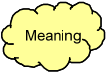
\includegraphics[width=20mm]{arquitectura/imagenes/113} \\
		\hline
		\centering\vspace{1.52mm}Valor & \vspace{1.52mm}El valor de pariente, utilidad, o importancia de un servicio de gestión o producto. & \vspace{1.52mm}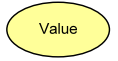
\includegraphics[width=25mm]{arquitectura/imagenes/114} \\
		\hline
		\centering\vspace{1.52mm}Producto & \vspace{1.52mm}Una colección coherente de servicios, acompañados por un contraer/poner de acuerdos, que ofrecen en total (a interno o externo) a clientes. & \vspace{1.52mm}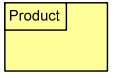
\includegraphics[width=20mm]{arquitectura/imagenes/115} \\
		\hline
		\centering\vspace{1.52mm}Contrato & \vspace{1.52mm}Una especificación formal o informal de acuerdo que especifica los derechos y obligaciones asociadas con un producto. & \vspace{1.52mm}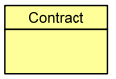
\includegraphics[width=20mm]{arquitectura/imagenes/116} \\
		\hline
	\end{tabular}
	\caption{Tabla de Conceptos de la Capa de Negocio}
	\label{fig:negocio}
\end{table}

\subsection{Capa de Aplicación}

Se trata de aplicaciones de software que "soportan los componentes de la empresa con servicios de aplicación".

\begin{table}[H]
	\centering\textbf{TABLA CONCEPTOS CAPA DE APLICACIÓN}
	\centering
	\begin{tabular}{| m{4cm} | m{4cm} | m{4cm} | }
		\hline
		\centering\vspace{1.52mm}CONCEPTO & \centering\vspace{1.52mm}DESCRIPCION &\vspace{1.52mm}NOTACION \\
		\hline
		\centering\vspace{1.52mm}Componente de Aplicación & \vspace{1.52mm}Una parte modular, desplegable, y reemplazable de un sistema de software que encapsula su comportamiento y datos y expone estos por un juego de interfaces.& \vspace{1.52mm}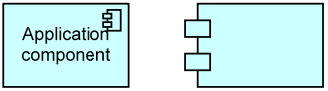
\includegraphics[width=40mm]{arquitectura/imagenes/21} \\
		\hline
		\centering\vspace{1.52mm}Colaboración de Aplicación & \vspace{1.52mm}Un conjunto de dos o más componentes de aplicación que trabajan juntos para realizar el comportamiento colectivo.& \vspace{1.52mm}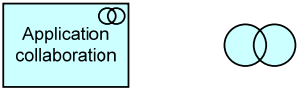
\includegraphics[width=40mm]{arquitectura/imagenes/22} \\
		\hline
		\centering\vspace{1.52mm}Interfaz de Aplicación & \vspace{1.52mm}Un punto de acceso donde un servicio de aplicación es hecho disponible a un usuario u otro componente de aplicación.& \vspace{1.52mm}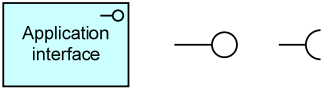
\includegraphics[width=40mm]{arquitectura/imagenes/23} \\
		\hline
		\centering\vspace{1.52mm}Objeto de Datos & \vspace{1.52mm}Un elemento pasivo conveniente para tratamiento automatizado.& \vspace{1.52mm}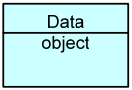
\includegraphics[width=20mm]{arquitectura/imagenes/24} \\
		\hline
		\centering\vspace{1.52mm}Función de Aplicación & \vspace{1.52mm}Un elemento de comportamiento que los grupos automatizaron el comportamiento que puede ser realizado por un componente de aplicación.& \vspace{1.52mm}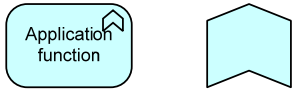
\includegraphics[width=40mm]{arquitectura/imagenes/25} \\
		\hline
		\centering\vspace{1.52mm}Interacción de Aplicación & \vspace{1.52mm}Un elemento de comportamiento que describe el comportamiento de una colaboración de aplicación.& \vspace{1.52mm}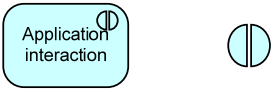
\includegraphics[width=40mm]{arquitectura/imagenes/26} \\
		\hline
		\centering\vspace{1.52mm}Servicio de Aplicación & \vspace{1.52mm}Un servicio que expone el comportamiento automatizado.& \vspace{1.52mm}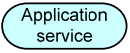
\includegraphics[width=20mm]{arquitectura/imagenes/27} \\
		\hline
	\end{tabular}
	\caption{Tabla de Conceptos de la Capa de Aplicación}
	\label{fig:aplicacion}
\end{table}

\subsection{Capa de Tecnologías}

Esta capa "Trata con la infraestructura de hardware y comunicación para soportar la Capa de Aplicación, esta capa ofrece servicios de infraestructura necesarios para ejecutar aplicaciones, realizadas por computadora y hardware de comunicación y software de sistema ".


\begin{table}[H]
	\centering\textbf{TABLA CONCEPTOS CAPA DE TECNOLOGIAS}
	\centering
	\begin{tabular}{| m{4cm} | m{4cm} | m{4cm} | }
		\hline
		\centering\vspace{1.52mm}CONCEPTO & \centering\vspace{1.52mm}DESCRIPCION &\vspace{1.52mm}NOTACION \\
		\hline
		\centering\vspace{1.52mm}Nodo & \vspace{1.52mm}Un recurso computacional con lo cual los artefactos pueden ser almacenados o desplegados para la ejecución.& \vspace{1.52mm}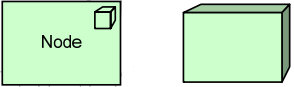
\includegraphics[width=40mm]{arquitectura/imagenes/31} \\
		\hline
		\centering\vspace{1.52mm}Dispositivo & \vspace{1.52mm}Un recurso de hardware con lo cual los artefactos pueden ser almacenados o desplegados para la ejecución.& \vspace{1.52mm}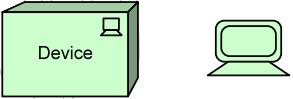
\includegraphics[width=40mm]{arquitectura/imagenes/32} \\
		\hline
		\centering\vspace{1.52mm}Red & \vspace{1.52mm}Un medio de comunicación entre dos o más dispositivos.& \vspace{1.52mm}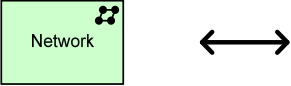
\includegraphics[width=40mm]{arquitectura/imagenes/33} \\
		\hline
		\centering\vspace{1.52mm}Camino de Comunicación & \vspace{1.52mm}Un eslabón entre dos o más nodos, por los cuales estos nodos pueden cambiar datos.& \vspace{1.52mm}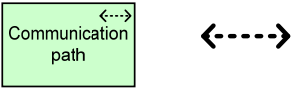
\includegraphics[width=40mm]{arquitectura/imagenes/34} \\
		\hline
		\centering\vspace{1.52mm}Interface de Infraestructura & \vspace{1.52mm}Un punto de acceso donde los servicios de infraestructura ofrecidos por un nodo pueden ser tenidos acceso por otros nodos y componentes de aplicación. & \vspace{1.52mm}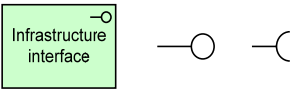
\includegraphics[width=40mm]{arquitectura/imagenes/35} \\
		\hline
		\centering\vspace{1.52mm}Sistema de Software & \vspace{1.52mm}Un entorno de software para los tipos específicos de componentes y objetos que son desplegados sobre ello en forma de artefactos.& \vspace{1.52mm}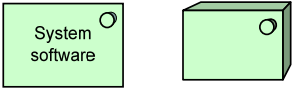
\includegraphics[width=40mm]{arquitectura/imagenes/36} \\
		\hline
		\centering\vspace{1.52mm}Función de Infraestructura & \vspace{1.52mm}Un elemento de comportamiento de grupos el comportamiento infraestructural puede ser realizado por un nodo.& \vspace{1.52mm}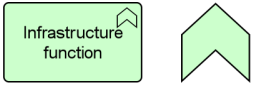
\includegraphics[width=40mm]{arquitectura/imagenes/37} \\
		\hline
		\centering\vspace{1.52mm}Servicios de Infraestructura & \vspace{1.52mm}Una unidad por fuera visible de funcionalidad, a condición de que por uno o varios nodos, expuestos por interfaces bien definidos, y significativo al entorno.& \vspace{1.52mm}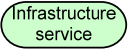
\includegraphics[width=20mm]{arquitectura/imagenes/38} \\
		\hline
	\end{tabular}
\end{table}

\begin{table}[H]
	\centering
	\begin{tabular}{| m{4cm} | m{4cm} | m{4cm} | }
		\hline
		\centering\vspace{1.52mm}CONCEPTO & \centering\vspace{1.52mm}DESCRIPCION &\vspace{1.52mm}NOTACION \\
		\hline
		\centering\vspace{1.52mm}Artefacto & \vspace{1.52mm}Un pedazo físico de los datos que es usado o producido en un proceso de desarrollo de software, o por el despliegue y la operación de un sistema.& \vspace{1.52mm}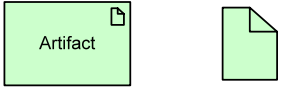
\includegraphics[width=40mm]{arquitectura/imagenes/39} \\
		\hline
	\end{tabular}
	\caption{Tabla de Conceptos de la Capa de Tecnologías}
	\label{fig:tecnologias}
\end{table}

\subsection{Capa de Motivación}

Los conceptos de motivación se utilizan para modelar las motivaciones, o razones, que subyacen en el diseño o cambio de alguna arquitectura empresarial. Estas motivaciones afectan, orientan y limitan el diseño.


\begin{table}[H]
	\centering\textbf{TABLA DE CONCEPTOS CAPA DE MOTIVACIÓN}
	\centering
	\begin{tabular}{| m{4cm} | m{4cm} | m{4cm} | }
		\hline
		\centering\vspace{1.52mm}CONCEPTO & \centering\vspace{1.52mm}DESCRIPCION &\vspace{1.52mm}NOTACION \\
		\hline
		\centering\vspace{1.52mm}Tenedor de Apuestas& \vspace{1.52mm}El papel de un individuo, el equipo, o la organización (o clasifica de eso) que representa sus intereses a, o concierne en relación con, el resultado de la arquitectura.& \vspace{1.52mm}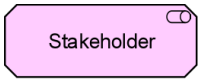
\includegraphics[width=30mm]{arquitectura/imagenes/51} \\
		\hline
		\centering\vspace{1.52mm}Conductor& \vspace{1.52mm}Algo qué crea, motiva, y abastece de combustible el cambio de una organización.& \vspace{1.52mm}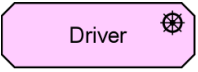
\includegraphics[width=30mm]{arquitectura/imagenes/52} \\
		\hline
		\centering\vspace{1.52mm}Evaluación& \vspace{1.52mm}El resultado de algún análisis de algún conductor.& \vspace{1.52mm}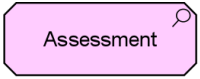
\includegraphics[width=30mm]{arquitectura/imagenes/53} \\
		\hline
		\centering\vspace{1.52mm}Objetivo& \vspace{1.52mm}Un estado de final que un tenedor de apuestas tiene la intención de alcanzar.& \vspace{1.52mm}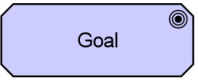
\includegraphics[width=30mm]{arquitectura/imagenes/54} \\
		\hline
		\centering\vspace{1.52mm}Requerimientos& \vspace{1.52mm}Una declaración de necesidad que debe ser realizada por un sistema.& \vspace{1.52mm}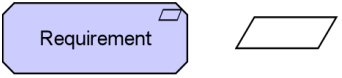
\includegraphics[width=40mm]{arquitectura/imagenes/55} \\
		\hline
		\centering\vspace{1.52mm}Coacción& \vspace{1.52mm}Una restricción en el camino en la cual un sistema es realizado.& \vspace{1.52mm}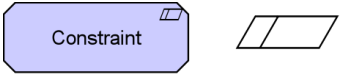
\includegraphics[width=40mm]{arquitectura/imagenes/56} \\
		\hline
		\centering\vspace{1.52mm}Principio& \vspace{1.52mm}Una propiedad normativa de todos los sistemas en un contexto dado, o el camino en cual ellos son realizados.& \vspace{1.52mm}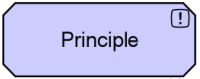
\includegraphics[width=30mm]{arquitectura/imagenes/57} \\
		\hline
	\end{tabular}
	\caption{Tabla de Conceptos de Capa Motivación}
	\label{fig:motivacion}
\end{table}

\subsection{Capa de Implementación y  Migración}

 Es similar a un proceso de negocio, en el sentido de que consiste en un conjunto de tareas relacionadas causalmente, dirigidas a producir un resultado bien definido.

\begin{table}[H]
	\centering\textbf{TABLA DE CONCEPTOS CAPA DE IMPLEMENTACIÓN Y MIGRACIÓN}
	\centering
	\begin{tabular}{| m{4cm} | m{4cm} | m{4cm} | }
		\hline
		\centering\vspace{1.52mm}CONCEPTO & \centering\vspace{1.52mm}DESCRIPCION &\vspace{1.52mm}NOTACION \\
		\hline
		\centering\vspace{1.52mm}Paquete de Trabajo& \vspace{1.52mm}Una serie de acciones diseñadas para lograr un objetivo único dentro de un tiempo especificado.& \vspace{1.52mm}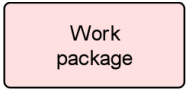
\includegraphics[width=25mm]{arquitectura/imagenes/61} \\
		\hline
		\centering\vspace{1.52mm}Entregable& \vspace{1.52mm}Un resultado definido con precisión de un paquete de trabajo.& \vspace{1.52mm}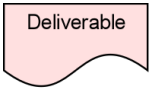
\includegraphics[width=20mm]{arquitectura/imagenes/62} \\
		\hline
		\centering\vspace{1.52mm}Meseta& \vspace{1.52mm}Un estado relativamente estable de la arquitectura que existe durante un período limitado de tiempo.& \vspace{1.52mm}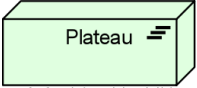
\includegraphics[width=25mm]{arquitectura/imagenes/63} \\
		\hline
		\centering\vspace{1.52mm}Objetivo& \vspace{1.52mm}Un resultado de un análisis de hueco entre dos mesetas.& \vspace{1.52mm}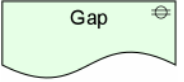
\includegraphics[width=25mm]{arquitectura/imagenes/64} \\
		\hline
	\end{tabular}
	\caption{Tabla de Conceptos de Capa Migración}
	\label{fig:migracion}
\end{table}

\subsection{Tabla de relaciones}

\begin{table}[H]
	\centering\textbf{TABLA DE RELACIONES}
	\centering
	\begin{tabular}{| m{4cm} | m{4cm} | m{4cm} | }
		\hline
		\centering\vspace{1.52mm}CONCEPTO & \centering\vspace{1.52mm}DESCRIPCION &\vspace{1.52mm}NOTACION \\
		\hline
		&\centering\vspace{1.52mm}RELACIONES ESTRUCTURALES & \\
		\hline
		\centering\vspace{1.52mm}Asociación & \vspace{1.52mm}La asociación modela una relación entre los objetos que no es cubierta por el otro, la relación más específica.& \vspace{1.52mm}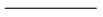
\includegraphics[width=40mm]{arquitectura/imagenes/41} \\
		\hline
		\centering\vspace{1.52mm}Acceso & \vspace{1.52mm}La relación de acceso modela el acceso de conceptos conductuales a objetos de datos o el negocio.& \vspace{1.52mm}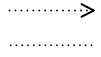
\includegraphics[width=40mm]{arquitectura/imagenes/42} \\
		\hline
		\centering\vspace{1.52mm}Usado Por & \vspace{1.52mm}El usado por la relación modela el empleo de servicios por procesos, funciones, o interacciones y el acceso a interfaces por papeles, componentes, o colaboraciones.& \vspace{1.52mm}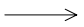
\includegraphics[width=30mm]{arquitectura/imagenes/43} \\
		\hline
	\end{tabular}
\end{table}

\begin{table}[H]
	\centering
	\begin{tabular}{| m{4cm} | m{4cm} | m{4cm} | }
		\hline
		\centering\vspace{1.52mm}CONCEPTO & \centering\vspace{1.52mm}DESCRIPCION &\vspace{1.52mm}NOTACION \\
		\hline
		\centering\vspace{1.52mm}Realización & \vspace{1.52mm}La relación de realización une una entidad lógica con más entidad concreta que lo realiza.& \vspace{1.52mm}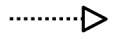
\includegraphics[width=30mm]{arquitectura/imagenes/44} \\
		\hline
		\centering\vspace{1.52mm}Asignación & \vspace{1.52mm}La relación de asignación une las unidades de comportamiento con elementos activos (p.ej., papeles, componentes) que los realiza, o papeles con los actores que los realizan.& \vspace{1.52mm}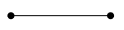
\includegraphics[width=30mm]{arquitectura/imagenes/45} \\
		\hline
		\centering\vspace{1.52mm}Agregación & \vspace{1.52mm}La relación de agregación indica que un objeto agrupa un número de otros objetos.& \vspace{1.52mm}\includegraphics[width=30mm]{arquitectura/imagenes/46} \\
		\hline
		\centering\vspace{1.52mm}Composición & \vspace{1.52mm}La relación de composición indica que un objeto es compuesto de uno o varios otros objetos.& \vspace{1.52mm}\includegraphics[width=30mm]{arquitectura/imagenes/47} \\
		\hline
		&\centering\vspace{1.52mm}RELACIONES DINAMICAS & \\
		\hline
		\centering\vspace{1.52mm}Flujo & \vspace{1.52mm}La relación de flujo describe la transferencia de, por ejemplo, la información o el valor entre procesos, función, interacciones, y acontecimientos.& \vspace{1.52mm}\includegraphics[width=30mm]{arquitectura/imagenes/48} \\
		\hline
		\centering\vspace{1.52mm}Provocación& \vspace{1.52mm}La relación de provocación describe las relaciones temporales o causales entre procesos, funciones, interacciones, y acontecimientos.& \vspace{1.52mm}\includegraphics[width=30mm]{arquitectura/imagenes/49} \\
		\hline
		&\centering\vspace{1.52mm}OTRAS RELACIONES & \\
		\hline
		\centering\vspace{1.52mm}Agrupación& \vspace{1.52mm}La relación que de agrupación indica que los objetos, del mismo tipo o tipos diferentes, pertenecen juntos basado en alguna característica común.& \vspace{1.52mm}\includegraphics[width=20mm]{arquitectura/imagenes/410} \\
		\hline
		\centering\vspace{1.52mm}Unión& \vspace{1.52mm}Una unión es usada para unir las relaciones del mismo tipo.& \vspace{1.52mm}\includegraphics[width=20mm]{arquitectura/imagenes/411} \\
		\hline
		\centering\vspace{1.52mm}Especialización& \vspace{1.52mm}La relación de especialización indica que un objeto es una especialización de otro objeto.& \vspace{1.52mm}\includegraphics[width=20mm]{arquitectura/imagenes/412} \\
		\hline
	\end{tabular}
	\caption{Tabla de Relaciones}
	\label{fig:relaciones}
\end{table}


\section{Intergación AMD y ArchiMate}

\begin{figure}[h]
	\centering
	\includegraphics[width=0.7\linewidth]{arquitectura/imagenes/AMD_ArchiMate}
	\caption{Relación entre AMD y ArchiMate \cite{togaf3}.}
	\label{fig:amdarchimate}
\end{figure}


Como se logra ver en la imagen la estructura del lenguaje central de ArchiMate se relaciona estrechamente con las arquitecturas principales de TOGAF ADM. Los elementos de estrategia, motivación, implementación y migración se correlacionan aproximadamente con el resto de ADM (aunque estos elementos también pueden usarse en las Fases B, C y D). Esta correspondencia indica una asignación bastante fácil entre las vistas TOGAF y los puntos de vista de ArchiMate.
\newline
Aunque algunos de los puntos de vista que se definen en el estándar TOGAF no se pueden asignar fácilmente a los puntos de vista de ArchiMate, el lenguaje ArchiMate y sus técnicas de análisis soportan los conceptos abordados en estos puntos de vista. Aunque no existe una correspondencia entre uno y otro, todavía hay una buena cantidad de correspondencia entre los puntos de vista de ArchiMate y los puntos de vista de TOGAF.
\newline
Los estándares de TOGAF y ArchiMate pueden usarse de forma fácil debido a que:

\begin{itemize}
	\item Los dos estándares se complementan entre sí con respecto a la definición de un proceso de desarrollo de arquitectura y la definición de un lenguaje de modelado de Arquitectura Empresarial.
	\item Las dos normas se superponen en su uso de los puntos de vista, y el concepto de un repositorio común subyacente de artefactos y modelos arquitectónicos; Es decir, tienen una base común firme.
	\item El uso combinado de las dos normas puede apoyar una mejor comunicación con las partes interesadas.
\end{itemize}


\newpage


